\documentclass{thesis}
% Class options: [singlespacing, onehalfspacing]

%%%%%%%%%%%%%%%%%%%%%%%%%%%%%%%%%%%%%%%%%%%%%%%%%%%%%%%%%%%%%%%%%%%%%%%%%%%%%%%
%% BASIC INFORMATION
%%%%%%%%%%%%%%%%%%%%%%%%%%%%%%%%%%%%%%%%%%%%%%%%%%%%%%%%%%%%%%%%%%%%%%%%%%%%%%%
\name{Cole}{Hengstebeck}
\title{Safety Critical Control of Simple Robotic Swarm Algorithms Using Control Barrier Functions}
\school{Miami University}
\college{Engineering and Computing}
\department{Electrical and Computer Engineering}
\location{Oxford}{Ohio}
\year{2023}

\listadd{\advisors}{Dr. Peter Jamieson}
\listadd{\advisors}{Dr. Bryan Van Scoy}
% \advisor1{Dr. Peter Jamieson}
% \advisor2{Dr. Bryan Van Scoy}
\listadd{\committee}{Dr. David Hartup}
\listadd{\committee}{Dr. Ran Zhang}


%%%%%%%%%%%%%%%%%%%%%%%%%%%%%%%%%%%%%%%%%%%%%%%%%%%%%%%%%%%%%%%%%%%%%%%%%%%%%%%
%% PACKAGES (not required)
%%%%%%%%%%%%%%%%%%%%%%%%%%%%%%%%%%%%%%%%%%%%%%%%%%%%%%%%%%%%%%%%%%%%%%%%%%%%%%%
\usepackage{lipsum}                   % filler text
\usepackage{graphicx}                 % figures
\usepackage{amsmath,amssymb,amsthm}   % mathematics
\usepackage{colonequals}              % for special := and =: symbols
\usepackage[shortlabels]{enumitem}    % customizable itemization
\usepackage{cite}                     % citation shortening
\usepackage{calc}                     % allows arithmetic with LaTeX lengths
\usepackage{booktabs}                 % pretty tables
\usepackage{multirow}
\usepackage{siunitx}
\usepackage{xcolor}
\usepackage{graphicx}
\usepackage{parskip}
\usepackage{thmtools}
\theoremstyle{definition}
\declaretheorem[name=Theorem, Refname={Theorem,Theorems}]{theorem}
\declaretheorem[name=Lemma, Refname={Lemma,Lemmas}, sibling=theorem]{lemma}
\declaretheorem[name=Corollary, Refname={Corollary,Corollaries}, sibling=theorem]{corollary}
\declaretheorem[name=Proposition, Refname={Proposition,Propositions}, sibling=theorem]{proposition}
\declaretheorem[name=Definition, Refname={Definition,Definitions}, sibling=theorem]{definition}
\declaretheorem[name=Theorem, Refname={Theorem,Theorems}, sibling=theorem,
			    shaded={bgcolor=black!20,margin=1ex,textwidth=\linewidth-2ex}]{theoremshaded}
\declaretheorem[name=Theorem, Refname={Theorem,Theorems}, sibling=theorem,
	            shaded={rulecolor=black, bgcolor=white, rulewidth=1pt, margin=1ex, textwidth=\linewidth-2ex-2pt}]{theoremboxed}

% more legible proof environment and QED symbol
\def\qed{\rule[0pt]{5pt}{5pt}\par\medskip}
\renewcommand{\qedhere}{\hfill ~\qed}
\renewenvironment{proof}{{\noindent\bf Proof.}}{\qedhere}

% customized figure captions
\usepackage[margin=10pt,font=small,labelfont=bf,labelsep=colon]{caption}
\captionsetup[figure]{name=Figure}
\captionsetup[table]{aboveskip=3pt}

% clever references (also for theorems and such)
\usepackage[capitalise,nameinlink]{cleveref}

% automatically look for graphics in these folders
\graphicspath{{graphics/}}


%%%%%%%%%%%%%%%%%%%%%%%%%%%%%%%%%%%%%%%%%%%%%%%%%%%%%%%%%%%%%%%%%%%%%%%%%%%%%%%
%% DEFINITIONS (not required)
%%%%%%%%%%%%%%%%%%%%%%%%%%%%%%%%%%%%%%%%%%%%%%%%%%%%%%%%%%%%%%%%%%%%%%%%%%%%%%%
\def\integer{\mathbb{Z}}                     % integers
\def\real{\mathbb{R}}                        % real numbers
\def\complex{\mathbb{C}}                     % complex numbers
\def\tp{\mathsf{T}}                          % tranpose
\def\Re{\mathrm{Re}}                         % real part of a complex number
\def\Im{\mathrm{Im}}                         % imaginary part of a complex number
\def\epsilon{\varepsilon}                    % epsilon
\def\defeq{\colonequals}                     % definitions
\def\eqdef{\equalscolon}                     % definitions
\def\grad{\nabla}                            % gradient
\DeclareMathOperator*{\argmin}{\arg\min}     % arg min
\DeclareMathOperator*{\argmax}{\arg\max}     % arg max
\DeclareMathOperator*{\minimize}{minimize}   % min
\DeclareMathOperator*{\maximize}{maximize}   % max
\DeclareMathOperator{\trace}{\mathrm{tr}}    % trace
\DeclareMathOperator{\diag}{\mathrm{diag}}   % diag

% MATRICES
\newcommand{\bmat}[1]{\begin{bmatrix}#1\end{bmatrix}}
\newcommand{\pmat}[1]{\begin{pmatrix}#1\end{pmatrix}}


%%%%%%%%%%%%%%%%%%%%%%%%%%%%%%%%%%%%%%%%%%%%%%%%%%%%%%%%%%%%%%%%%%%%%%%%%%%%%%%
%% MAIN DOCUMENT
%%%%%%%%%%%%%%%%%%%%%%%%%%%%%%%%%%%%%%%%%%%%%%%%%%%%%%%%%%%%%%%%%%%%%%%%%%%%%%%
\begin{document}

\frontmatter


%%%%%%%%%%%%%%%%%%%%%%%%%%%%%%%%%%%%%%%%%%%%%%%%%%%%%%%%%%%%%%%%%%%%%%%%%%%%%%%
%% ABSTRACT (200 word max, one paragraph)
%%%%%%%%%%%%%%%%%%%%%%%%%%%%%%%%%%%%%%%%%%%%%%%%%%%%%%%%%%%%%%%%%%%%%%%%%%%%%%%
\begin{abstract}
  This document is a template and guide for writing a thesis in \LaTeX. The document is divided into sections explaining the preferred way of typesetting equations, figures, tables, and more. To prepare your thesis, simply edit the file \texttt{thesis.tex} along with the chapters in the \texttt{chapter/} folder. To make the final pdf, open a command prompt, navigate to the folder containing the template, and run the following commands:
  
  \texttt{pdflatex thesis.tex}\\
  \texttt{bibtex thesis.aux}\\
  \texttt{pdflatex thesis.tex}\\
  \texttt{pdflatex thesis.tex}
\end{abstract}


%%%%%%%%%%%%%%%%%%%%%%%%%%%%%%%%%%%%%%%%%%%%%%%%%%%%%%%%%%%%%%%%%%%%%%%%%%%%%%%
%% TITLE AND SIGNATURE PAGE
%%%%%%%%%%%%%%%%%%%%%%%%%%%%%%%%%%%%%%%%%%%%%%%%%%%%%%%%%%%%%%%%%%%%%%%%%%%%%%%
\maketitle

% the title page is the first numbered page (not the abstract),
% but the first page number appears on the table of contents
\setcounter{page}{3}

% table of contents
\tableofcontents

% list of tables
\lot

% list of figures
\lof

% dedication (optional)
\chapter{Dedication}

I would like to dedicate this thesis to\ldots

% acknowledgements (optional)
\chapter{Acknowledgements}

I would like to acknowledge\ldots


%%%%%%%%%%%%%%%%%%%%%%%%%%%%%%%%%%%%%%%%%%%%%%%%%%%%%%%%%%%%%%%%%%%%%%%%%%%%%%%
%% CHAPTERS
%%%%%%%%%%%%%%%%%%%%%%%%%%%%%%%%%%%%%%%%%%%%%%%%%%%%%%%%%%%%%%%%%%%%%%%%%%%%%%%
\mainmatter
\chapter{Introduction}
\label{sec:intro}

Across many disciplines, in businesses, government projects, and academia, robots are being used to improve efficiency of certain tasks. Robots have been invited into our homes to clean the floors, entertain children in the form of toys, and mow our lawns.  In manufacturing and goods movement, robots are performing many tasks to improve these needed tasks.  Robotics is a broad field that includes countless form factors and abilities. One growing field of research and development within robotics is multi-agent systems and swarm robotics.

Swarm robotics is the control of multiple robots, also known as agents, in a manner that simulates the logic and movement of a swarm of biological animals or insects. These agents have individual control of themselves, but collaborate with their neighbors to accomplish a common goal. In swarm applications, the robots are able to move autonomously and are simple in design, often with only a few necessary sensors and actuators. The simplicity of their design allows swarms of robots to be more easily scaled in size and maintained.

Swarm robotics combines multi-agent systems with swarm intelligence. Swarm intelligence refers to emergent behavior similar to biological swarms, such as insects, fish, and birds, that gather information from their own senses and the interactions they have with their neighbors, but do not possess any omnipotent knowledge of the world around them. This is applied to algorithms that mimic these biological features onto a group of agents working within the same system.

Many applications for swarms of robots are emerging and have been proposed \cite{spezzano2019special}. Common uses for swarms of robots are to perform tasks in places where humans cannot or should not go. Examples of these applications are detecting chemical leaks, search and rescue in dangerous terrain, and working in radioactive environments. Industrial robots are also being used to replace humans in very repetitive, simple, or labor-intensive tasks, and swarms of robots are no different. Swarms are being used in warehouses to move products \cite{poudel2013coordinating} and on farms \cite{spezzano2019special} to increase the amount of simultaneous work that is able to be done.

Across all real-world robotics systems, safety is a central concern during the design and implementation of a system. ``Safety" can have different meanings depending on context. A robot may need to be gentle and precise when manipulating manufactured goods, avoid destruction to the physical environment and infrastructure in which it works, avoid risk to human life and injury, and prevent damage to itself and other robots it interacts with. Safety-critical systems are systems in which faults and failures can result in significant damage to any of the aforementioned areas \cite{knight2002safety}, with systems posing a risk to human safety being the most critical. There are many ways to make systems safe through hardware, software, and infrastructure, with more critical systems implementing more layers of safety. 

\section{Proposed Research}

Our research seeks to implement a swarm algorithm, in simulation and on a real-world system, and analyze the efficacy of the algorithm to keep the swarm safe. We extend a swarming algorithm with control barrier functions to make comparisons between the two algorithms in an attempt to make a simple algorithm safety-critical. Many algorithms have been developed to implement a swarm in simulation, real-world, or both. One simple algorithm is the Boids Algorithm developed by Craig Reynolds in 1987 \cite{reynolds1987flocks}, also called the Reynolds Boids or Reynolds Algorithm. This algorithm simulates the flocking behavior of birds by combining three base actions described by Reynolds: Separation, Alignment, and Cohesion. The effects of each parameter and a more in-depth explanation of the Boids Algorithm can be found in Chapter \ref{ch:back}, Section \ref{sec:boids}. The Boids Algorithm has been applied to robot control in many scenarios \cite{kasmarik2020autonomous,clark2012flight,jakimovski2008swarm}, both in simulation and on physical systems, and this thesis will do the same. 

This thesis aims to create a safety-critical swarm system using a simple base algorithm and extending it. The Boids Algorithm is the base algorithm for the control of our swarm, chosen for its relatively simple control paradigm. Our research aims to investigate the safety of this simple control algorithm as compared to an extended version of Boids (which we call Extended\_Boids) and a version of Boids modified to include control barrier functions. Speed, both in terms of time for the swarm to complete its task and the computational time to simulate, as well as the number of agents that reach their goal without a collision, is studied for comparing our algorithms. The safety goal is to achieve all agents at their destination without any collisions between two agents, an agent and the boundaries, or an agent and an obstacle. 

There are three systems we will investigate and compare. First, is the Boids Algorithm as described by Reynolds \cite{reynolds1987flocks} that just has agents flock without purpose. Second, the Extended\_Boids Algorithm that uses the same three rules, but with added functionality by adding what we call ``ghost boids" or ATONs (Aids TO Navigation). Ghost boids do not move but have influence on the movement of other boids, allowing an invisible influence that can be used to add obstacle avoidance and goal-seeking by positioning the ghost boids in certain locations, all without modifying the control algorithm. Lastly, we implement control barrier functions on top of the Extended\_Boids Algorithm which then allows the boids to act normally unless they are approaching unsafe conditions, at which point the control will begin to focus more on safety. We will investigate the performance of all three systems and compare them. After doing this in simulation, we aim to implement these algorithms on a physical swarm to investigate the success of the algorithms in a real-world environment.

\section{Contributions Of Our Work}

Our work has three main contributions:
\begin{enumerate}
    \item The novel use of ATONs and ghost boids to extend the Boids Algorithm to include goal-seeking and obstacle avoidance without modifying the base algorithm.
    \item The creation of a safety-critical swarm system that can be implemented in simulation or a real system through the use of control barrier functions.
    \item A methodology to analyze and compare of the performance of these algorithms.
\end{enumerate}

\section{Organization}

%Swarm robotics is an ever-growing section in the field of robotics. With applications in business, academia, and government environments, swarms of robots have individual control and autonomy, but collaborate for a common goal. Mimicking the behavior of biological swarms, robot swarms are usually simple in design to be low in cost and scalable. Our research investigates the safety-critical control of a robot swarm by simulating algorithms built on top of a simple control algorithm, the Boids Algorithm. Lastly, the algorithms will be implemented on a physical swarm of robots to investigate their real-world successes and failures.
The remainder of this thesis is organized as follows. In Chapter \ref{ch:back}, we provide the relevant background and state of the art. In Chapter~\ref{ch:3} Section~\ref{sec:work}  we discuss the progress we have made in this work. Finally, in Section \ref{sec:future} we provide a description of the work we will do to complete this thesis and a timeline for the proposed work.
\chapter{Background}
\label{ch:back}

In this section, we discuss some of the necessary background information needed for our work and work done by others that are is related to our project.

\section{Multi-Agent Systems}

Multi-agent systems, or multi-robot systems, are environments where multiple agents are working and interacting with each other. These systems rely on communication between agents in some manner to complete tasks and maintain safety. Multi-agent systems are not necessarily all homogeneous agents, meaning there can be different types of robots that are specialized for different tasks all operating in the same space and working together. We will discuss two existing multi-agent systems, the Kilobot and the Robotarium.

\subsection{Kilobot}

Developed by Harvard University, the Kilobot is a very low-cost agent that is capable of demonstrating swarm behavior \cite{rubenstein2014kilobot}. The Kilobot costs 14 USD in parts and thus can be scaled up to thousands of agents. The agents use two vibration motors to move in the direction they want and use infrared transmitters and receivers to reflect light off a table in order to communicate. Using the intensity detected by the infrared sensor, the agent is able to determine the distance it is from its neighbors. However, this does not allow an agent to know in which direction its neighbors are facing, and they have no knowledge of their global position in the workspace. An ambient light sensor and LED sit on top of the Kilobot to allow light-seeking algorithms to be implemented and communication to the human operators, respectively. 

The lack of wheels on the Kilobot results in a novel method of locomotion in mobile robots. It is common for mobile robots to utilize two wheels in a differential drive configuration to maneuver around its environment. However, the use of much smaller vibration motors is used to keep size and cost low. The benefits in size and cost, are traded off for in a robots achievable velocity. The Kilobots are able to move 1cm/s and rotate 45\textdegree/s \cite{rubenstein2014kilobot}. Differential drive robots are able to move faster than this, with actual speeds dependant on the motors used. 

The Kilobots have the ability to move around and communicate, which is needed to perform several collaborative tasks. In \cite{rubenstein2014kilobot}, the agents were able to demonstrate:
\begin{enumerate}
    \item Foraging (Finding ``food" and returning it to the ``nest"). The agents are able to explore and can enter a ``beacon" mode that remains stationary and communicate its distance from the food or nest in units of agents in the chain. Moving agents are able to follow the chain of beacons to get between the nest and food source.
    \item Formation Control (Follow-the-leader). One leader moves forward while other agents follow in a line. To make up for the lack of knowledge on the bearing of their neighbors, agents move forward-left and forward-right and sense which movements move them closer to their neighbors.
    \item Photoaxis (Move toward a light source). Using the light sensor to detect when the agent is moving closer or further from the light, the agents move in sweeping movements to reach the destination. The paper does not describe any use of communication for this example, but it could be used for collision avoidance.
    \item Synchronization. Each agent is given a random clock cycle and communicates to its neighbors when it completes a cycle. The neighbors adjust their own clock when they receive a signal, and over time all the agents are able to synchronize their clocks. This is useful for systems like this where there can be delays in communication.
\end{enumerate}

The research done by this team demonstrates some of the core characteristics of swarm robotics, namely the emphasis on low-cost, simple, and highly scalable agents. The Kilobots use very simple sensors and actuators but are able to demonstrate dynamic emergent behaviors. And at a low cost, they are able to conduct experiments with 100 individual agents. In later work shown in \cite{rubenstein2014programmable}, 1024 Kilobot agents are used to form large shapes, truly showing the scale swarms can take.
 
\subsection{Robotarium}
\label{sec:robotarium}

While agents developed for a swarm are intentionally simple and scalable, that does not mean it is simple to create a system capable of swarm control. Limitations in funding, space, experience, and necessity can prevent researchers from creating their own swarm of robots to run real-world tests. To help the academic community, The Georgia Institute of Technology has created the Robotarium, a free-access testbed for swarm robotics \cite{wilson2020robotarium}. Users can create a free account, write their own control algorithms in MATLAB or Python using the custom API, simulate and submit their code, and the algorithm is run on a physical swarm of robots and a video is returned of the agents moving. 

The system uses eight motion capture cameras and unique marker designs on the robots to track their movements. Using an overhead projector pointing down on the table, the Robotarium is able to display graphics, animations that follow agents, and system information in real time directly onto the tabletop. By mounting inductive chargers along the perimeter of the testbed, the robots are able to automatically charge themselves when not in use. By default, control barrier functions are built on top of the algorithms submitted by users to ensure safe control of the agents without collisions, though this can be disabled after review of submitted control algorithms. All of this allows the whole system to run automatically, during all hours of the day.

The robots used in the Robotarium are an updated version of the GRITSBot \cite{pickem2015gritsbot}, the GRITSBot X. The GRITSBot X is designed with two differential drive wheels, Wi-Fi communications, an induction charging receiver, and from figures in \cite{wilson2020robotarium}, it can be seen that they are mounted with several infrared distance sensors. The Robotarium has a swarm size of 22 agents, but not all of them have to be used; some agents can be charging on the perimeter if a simulation does not require them. Control algorithms can be very simple or very complex, all dependant on the user's needs. This system allows people across the world to use state-of-the-art technology for academic purposes, all for free.

\section{Swarming and Flocking Algorithms}

In this thesis, there is a focus on swarming and flocking within a multi-agent system. Swarming is when a group of agents is moving in a cohesive group in some manner. There can be one large swarm of agents which includes all agents in the system, or there can be several smaller groups of agents that are swarming in individual ways. Flocking is a form of swarming that refers to the motion of birds as they fly in a flock. This section looks at several swarming algorithms with an emphasis on flocking algorithms.

\subsection{Reynolds Boids}
\label{sec:boids}

Originally developed in 1987 to simulate flocks of birds in computer animation, the algorithm by Craig Reynolds \cite{reynolds1987flocks} describes the motion of ``bird-oid" objects called boids. The Reynolds Boids, or simply, Boids Algorithm describes a flock not by its motion as a whole but through the emergent behavior that comes from each individual boid acting according to its limited perception of the environment around it. This mimics real birds that have limited knowledge and act on that knowledge individually to form flocks. This allows swarms of boids to scale in size easily for ease of animation or programming.

The algorithm relies on three weighted rules to modify the heading of a boid, which then moves with constant speed in that direction. The three rules are: 

\begin{enumerate}
    \item Collision Avoidance, often called \textbf{Separation} - Avoid colliding with other boids
    \item Velocity Matching, often called \textbf{Alignment} - Attempt to match the heading of nearby boids
    \item Flock Centering, often called \textbf{Cohesion} - Attempt to stay with the flock by moving towards the center of mass of nearby boids
\end{enumerate}

These three rules can be visualized in Figure \ref{fig:boids_rules} where the current boid is in red and can only see other boids within its radius. Boids inside the radius are blue and affect the motion of the current boid, all other boids are gray. The vector in green is the direction in which the specific rule will influence the boid. After the direction of each rule is calculated, different weights/scalars can be given to each rule to give more or less influence on the motion of the boid. Lastly, each weighted rule is combined with the current heading to form the new heading of the boid. This process is repeated for all boids to create the flocking motion.

\begin{figure}[h]
    \centering
    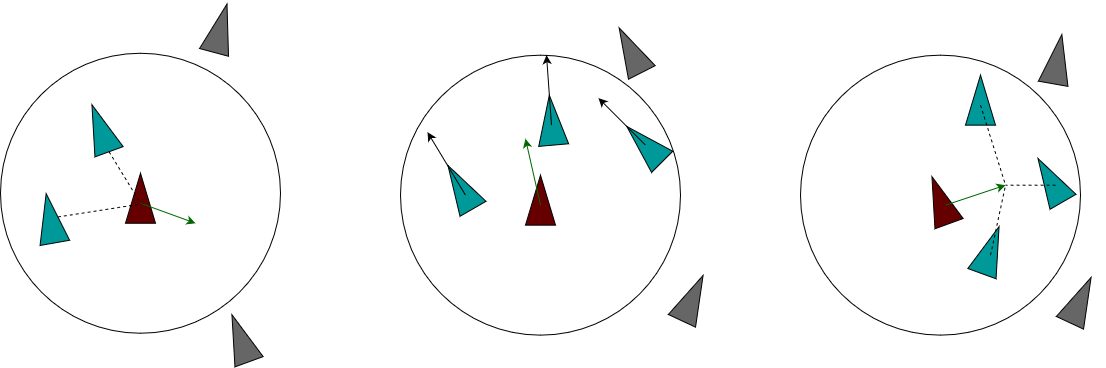
\includegraphics[width=\textwidth]{Figures/boids_rules.png}
    \caption{Visualization of Boids rules. From left to right, separation, alignment, and cohesion rules.}
    \label{fig:boids_rules}
\end{figure}

\subsection{Boid Guidance Algorithms}

Although Boids was created for computer animations, the Boids Algorithm can be applied to any multi-agent environment, including robotics. However, the Boids Algorithm only has rules to avoid other boids, not general obstacles, and has no means to have goals. The team in \cite{clark2012flight} use two additional rules to make this possible. The target seeking and obstacle avoidance rules are added to the algorithm and are weighted and included in the sum of rules just as separation, alignment, and cohesion are. This allows the agents of the swarm to be more safe and to complete tasks. This algorithm was then implemented on UAVs (Unmanned Ariel Vehicles).

The proposed system is made more dynamic by including a lookup table of rule weights that change dependant on different flags raised during execution. For example, as two boids move closer to each other, the internal flags of the agents change and the weight for the separation rule are increased to prioritize avoiding a collision. Work in \cite{crowther2004rule} did this using continuous functions rather than a lookup table of values, however the work in \cite{clark2012flight} had limitations on computational resources onboard the UAVs. The dynamic weights enable the algorithm to better optimize the control of the agent dependant on the environment it perceives. Lastly, to ensure the UAV does not leave the boundaries of the experiment, when within a certain distance to a border, control is given entirely to a boundary avoidance command that moves the agent directly orthogonal to the boundary for a certain distance. During this time there is no flocking or goal seeking control happening. This was a decision by the team to prioritize safety of the public outside the testing environment and this approach is a trade off they were chose to make.

\subsection{BEECLUST}

Birds are not the only biological animal that has been emulated with algorithms. By observing the movements of actual bees, Schmickl, a zoologist, and Hamann, an engineer, \cite{schmickl2011beeclust} were able to discover some of the walking patterns of bees and recreate them in robotic algorithms. They called their bee swarming algorithm -  BEECLUST. They found that some of the movements of bees depend on the temperature of the area the bees are standing in. Their algorithm has the following five properties, but in their system they replaced differing temperatures with varying light intensities that the agents are able to sense.

\begin{enumerate}
    \item The agent moves forward until it encounters an obstacle.
    \item If the obstacle is not another agent, it turns away and goes back to step 1.
    \item If the obstacle is another agent, the agent stops moving and measures the light intensity.
    \item The more intense the light (i.e. more heat), the robot will stay stationary for a longer time.
    \item After the waiting time, the agent turns away from the other robot and goes back to step 1.
\end{enumerate}

Through these properties, agents tend to cluster together around areas of higher light. This is a means of swarm formation as the agents group together without any means of communication between them. This algorithm was implemented in simulation and on a real swarm system and both showed the same pattern of many agents swarming in areas of higher light.

\section{Safety-Critical Control}

Safety-critical systems is a broad term and whether or not a system is safety-critical relies entirely on the specific context of the system. Safety-critical systems are systems whose failure can cause significant risk to human safety, incur economic losses, or pose a danger to the environment around the system, whether natural or artificial. In the context of this thesis, safety-critical systems refers to the computer and electronic systems that ensure safety, although there are non-computer safety measures that mitigate risk such as using barriers or nets. 

The work by Knight, et al. in \cite{knight2002safety} provides several examples of safety-critical systems, some less obvious than others. The Boeing 777 airplane, for example, has three separate channels for control, all to complete the same goal, but utilizing different equipment in isolation from each other to provide layers of redundancy in case one channel fails. Examples like this shows a clear danger to human life if critical systems fail, but there are other safety critical systems that aren't focused on human safety. Banking systems have redundancies and checks to ensure financial safety, and telecommunications systems have elements to maintain service to the best degree and shorten down-times if there is a fault.

As computers are being added to more and more devices, many new types of devices need to consider safety-critical design. Cheng, et al. \cite{cheng2019nn} develop safety-critical systems in self driving cars using neural networks. These systems have to account for a far greater number of events than ever required in cars. Self driving cars are not just an example of how systems need to be robust and reliable enough to prevent harm, safety systems are also required to develop the technology by getting the trust and support of the public. If self driving cars, or any other example, cannot be trustworthy in the eyes of the general population, these new technologies will be more heavily regulated in law, not be purchased and profitable, and research and development will not be funded.

In a survey on safety applications in robotics, \cite{guiochet2017safety} describes four means to avoiding risk:

\begin{enumerate}
    \item Fault Prevention - Practices that lower the chance of a fault occurring to begin with. Proper techniques, practices, and diligence are the foundation of prevention.
    \item Fault Removal - Verifications and validations that reveal and remove faults prior to system implementation.
    \item Fault Forecasting - Estimating and predicting the commonality of certain faults from happening and the severity of the consequences caused by the faults. Risk analysis is a large part of fault forecasting.
    \item Fault Tolerance - Redundancies and error detection that recognize a fault and prevent or mitigate the risk associated with the fault.
\end{enumerate}

\subsection{Control-Barrier Functions}

In robotics systems, there is often a trade off between task performance and safety. When a robot system is required to act more safe, it usually hinders its ability to move and complete a task in the most efficient way possible. The acceptable risk is determined by system designers, and certain systems can trade performance for safety in different ways. Control barrier functions \cite{ames2019control} are growing in popularity as a way to balance task-oriented control and safety-critical control within an agent. In implementing control barrier functions, a set of safe system states is defined, and the complement is the unsafe set. While operating well within the safe set, control can be almost entirely given to the task-oriented system. However, as the agent approaches the unsafe set, the control barrier function starts to enforce staying within the safe set, known as enforcing invariance. Control barrier functions are minimally invasive by design. The control barrier function provides the least disruptive control to the agent that enforces invariance. As the state of the agent enters deeper into the safe set, more control is returned to completing tasks. The use of control barrier functions and control barrier certificates ensures the agent operates only within the safe set and thus ensures the system is safety-critical.

\subsection{Aids To Navigation}

Aids To Navigation, or ATONs for short, are nautical buoys, lighthouses, and other markings to indicate dangerous areas that vessels should avoid \cite{CoastGuard}. ATONs are colored and shaped in different ways to indicate different types and sizes of danger. The two types that are pertinent to this thesis are the cardinal marks and isolated danger marks. Cardinal marks define the boundary of a large area to avoid, such as a reef. Isolated danger marks signal that there is a smaller danger to be avoided, such as a piece of debris on the seabed. In the context of this thesis, we use the nomenclature of cardinal marks to define the boundary of the workspace and isolated danger marks for individual obstacles in the test environment.


%%%%%%%%%%%%%%%%%%%%%%%%%%%%%%%%%%%%%%%%%%%%%%%%%%%%%%%%%%%%%%%%%%%%%%%%%%%%%%%
%% APPENDICES
%%%%%%%%%%%%%%%%%%%%%%%%%%%%%%%%%%%%%%%%%%%%%%%%%%%%%%%%%%%%%%%%%%%%%%%%%%%%%%%
\appendices


\backmatter


%%%%%%%%%%%%%%%%%%%%%%%%%%%%%%%%%%%%%%%%%%%%%%%%%%%%%%%%%%%%%%%%%%%%%%%%%%%%%%%
%% BIBLIOGRAPHY
%%%%%%%%%%%%%%%%%%%%%%%%%%%%%%%%%%%%%%%%%%%%%%%%%%%%%%%%%%%%%%%%%%%%%%%%%%%%%%%
\addcontentsline{toc}{chapter}{References}
\renewcommand\bibname{References}
\bibliography{references}

\end{document}